
As the rocket burns fuel the fill level of the tanks will decrease resulting in a change of center of gravity and inertia. To model this affect, functions for each of the subrocket are created to output the center of gravity and inertia as a function of fuel consumption. First, the rocket is sized and each independent stage's inertia and center of gravity of functions are found, then combined for the subrockets.

\textbf{Tank sizing}: the tanks are sized assuming cylindrical tanks, the constants of \autoref{tab:tank_sizing_constants} are used in \autoref{eq:tank_sizing} to give the height of tanks and the mass of the fluid within them. The results are displayed in \autoref{tab:tank_sizing_results}.

\begin{equation}
\begin{aligned}
    m_{LOX} =& \frac{m_{prop}}{\frac{O}{F}} \\
    m_{LCH_4} =& m_{prop} - m_{LOX} \\
    h_f =& \frac{m_{LCH_4}}{\rho_{LCH_4}} \cdot \frac{1}{\pi \cdot (r_r - t_{wall})^2} \\
    h_{ox} =& \frac{m_{LOX}}{\rho_{LOX}} \cdot \frac{1}{\pi \cdot (r_r - t_{wall})^2}
\end{aligned}
\label{eq:tank_sizing}
\end{equation}

\begin{table}[H]
    \centering
    \begin{minipage}{0.45\textwidth}
        \centering
        \caption{Tank sizing constants}
        \begin{tabular}{|c|c|}
             \hline
             Variable [unit] & Value \\ \hline
             $\rho_{LOX}$ [$kg/m^3$] & 1200 \\
             $\rho_{LCH_4}$ [$kg/m^3$] & 450 \\
             $\frac{O}{F}$ [$-$] & 3.545 \\
             $t_{wall}$ [$m$] & 0.01 \\
             \hline
        \end{tabular}
        \label{tab:tank_sizing_constants}
    \end{minipage}%
    \hspace{0.05\textwidth}
    \begin{minipage}{0.45\textwidth}
        \centering
        \caption{Tank sizing results}
        \begin{tabular}{|c|c|c|}
            \hline
             Variable [unit] & Stage 1 & Stage 2 \\ \hline
             $m_{LOX}$ [$kg$] & - & - \\
             $m_{LCH_4}$ [$kg$] & - & - \\
             $h_{LOX}$ [$m$] & - & - \\
             $h_{LCH_4}$ [$m$] & - & - \\ \hline
        \end{tabular}
        \label{tab:tank_sizing_results}
    \end{minipage}
\end{table}

\textbf{Stage sizing procedure}

The 2 stage rocket was divided into sections, as shown in \autoref{fig:rocket_sections} to determine the center of gravity and inertia through low fidelity sizing. This is not an accurate, however is representative of change in inertia a rocket might experience. The first stage has four structural mass components, a lower and upper section containing avionics equipment, stage and engine adapters, and the tank's structural walls and engines themselves. The second stage replaces has an additional payload and nose section.

\begin{figure}[H]
    \centering
    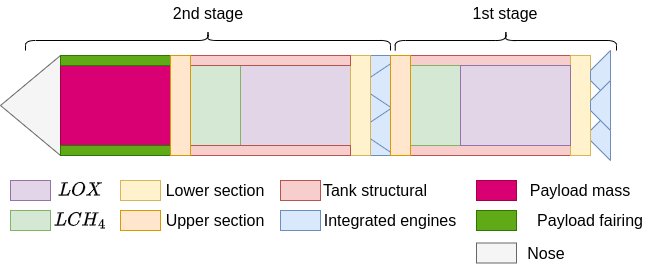
\includegraphics[width=0.95\linewidth]{figures/LiteratureStudy/RocketDiagram_new_new.png}
    \caption{Sectioning of rocket}
    \label{fig:rocket_sections}
\end{figure}

\textbf{First stage dry inertia}: The masses of each of the first stage are calculated through \autoref{eq:stage_masses_1}, using cylindrical tanks. The $\Lambda_{ul}$ is the factor of mass remaining structural mass distribution between the upper and lower section height.

\begin{equation}
\begin{aligned}
    m_{s,tanks} =& \pi \cdot (h_f + h_{ox}) \cdot (r_r^2 - (r_r - t_{wall})^2) \cdot \rho_{304L} \\
    m_{e,stage} =& n_e \cdot m_{e,integrated} \\
    m_{upper} =& (m_s - m_{s,tanks} - m_{e,stage}) \cdot \frac{1}{1 + \Lambda_{ul}} \\
    m_{lower} =& (m_s - m_{s,tanks} - m_{e,stage}) \cdot \frac{\Lambda_{ul}}{1+\Lambda_{ul}}
\end{aligned}
\label{eq:stage_masses_1}
\end{equation}

\begin{equation}
\begin{aligned}
    h_{upper} =& \frac{m_{upper}}{\rho_{upper}} \cdot \frac{1}{\pi \cdot r_r^2} \\
    h_{lower} =& \frac{m_{lower}}{\rho_{lower}} \cdot \frac{1}{\pi \cdot r_r^2} \\
\end{aligned}
\label{eq:section_heights}
\end{equation}

\begin{equation}
    x_{dry} = \frac{-m_{e,stage} \cdot \frac{h_e}{2} + m_{lower} \cdot \frac{h_{lower}}{2} + m_{s,tanks} \cdot (h_{lower} + \frac{h_f + h_{ox}}{2}) + m_{upper} \cdot (h_{lower} + h_f + h_{ox} + \frac{h_{upper}}{2})}{m_s}
\label{eq:dry_cog}
\end{equation}

Now the dry inertia is calculated using the cylinder moment of inertia equation

\begin{equation}
\begin{aligned}
    I_{e,stage} =& \frac{1}{12} \cdot m_{e,stage} \cdot h_e^2 - m_{e,stage} \cdot (x_{dry} + \frac{h_e}{2})^2 \\
    I_{lower} =& \frac{1}{12} \cdot m_{lower} \cdot h_{lower}^2 + m_{lower} \cdot (\frac{h_{lower}}{2} - x_{dry})^2 \\
    I_{upper} =& \frac{1}{12} \cdot m_{upper} \cdot h_{upper}^2 + m_{upper} \cdot (h_{lower} + h_{ox} + h_f + \frac{h_{upper}}{2} - x_{dry})^2 \\
    I_{s,tanks} =& \frac{1}{12} \cdot m_{s,tanks} \cdot (h_f + h_{ox})^2 + m_{s,tanks} \cdot (h_{lower} + \frac{h_f + h_{ox}}{2} - x_{dry})^2 \\
    I_{dry} =& I_{e,stage} + I_{lower} + I_{upper} + I_{s,tanks}
\end{aligned}
\label{eq:dry_inertia_1}
\end{equation}

\textbf{Second stage dry moment of inertia}: The payload structural mass is first computed using \autoref{eq:payload_strc}, alike to the tank structural masses. \autoref{eq:stage_masses_1} is used to get the stage's total integrated engines mass, and the tank structural mass. Using the volume of cone the nose mase is calculated in \autoref{eq:dry_2} allowing for the left-over mass to be applied to the second stage's lower and stages.

\begin{equation}
\begin{aligned}
    h_{pay} =& \frac{m_{pay}}{\rho_{pay}} \cdot \frac{1}{\pi \cdot (r_r - t_{fairing})^2} \\
    m_{s,pay} =& \pi \cdot h_{pay} \cdot (r_r^2 - (r_r - t_{fairing})^2) \cdot \rho_{304L}
\end{aligned}
\label{eq:payload_strc}
\end{equation}

\begin{equation}
\begin{aligned}
    m_{s,nose} =& \frac{1}{3} \cdot \pi r_r^3 \cdot \rho_{nose}\\
    m_{s,upper} =& (m_s - m_{s,pay} - m_{s,tanks} - m_{e,stage} - m_{s,nose}) \cdot \frac{1}{1 + \Lambda_{ul}}\\
    m_{s,lower} =& (m_s - m_{s,pay} - m_{s,tanks} - m_{e,stage} - m_{s,nose}) \cdot \frac{\Lambda_{ul}}{1 + \Lambda_{ul}}\\
\end{aligned}
\label{eq:dry_2}
\end{equation}

The dry center of gravity for the second stage including payload mass becomes:

\begin{equation}
\begin{aligned}
    x_{cog} =& [-m_{e,stage} \cdot \frac{h_e}{2} + m_{lower} \cdot \frac{h_{lower}}{2} + m_{s,tank} \cdot (h_{lower} + \frac{h_f + h_{ox}}{2}) \\
    +& m_{upper} \cdot (h_{lower} + h_f + h_{ox} + \frac{h_{upper}}{2}) + (m_{pay} + m_{s,pay}) \cdot (h_{lower} + h_f + h_{ox} + h_{upper} +  \frac{h_{pay}}{2}) \\
    +& m_{nose} \cdot (h_{lower} + h_f + h_{ox} + h_{upper} + h_{pay} + \frac{r_r}{8}] \cdot \frac{1}{m_s + m_{pay}}
\end{aligned}
\end{equation}


Now the dry moment of inertia can be found, taking $I_{e,stage}$, $I_{lower}$, $I_{upper}$ and $I_{s,tanks}$ from \autoref{eq:dry_inertia_1}.

\begin{equation}
\begin{aligned}
    I_{pay} =& \frac{1}{12} \cdot (m_{pay} + m_{s,pay}) \cdot  h_{pay}^2 + (m_{pay} + m_{s,pay}) \cdot (h_{lower} + h_f + h_{ox} + h_{upper} + \frac{h_{pay}}{2} - x_{dry})^2 \\
    I_{nose} =& \frac{3}{80} \cdot m_{s,nose} \cdot (5 \cdot r_r^2) + m_{s,nose} \cdot (h_{lower} + h_f + h_{ox} + h_{upper} + h_{pay} + \frac{r_r}{4} - x_{dry})^2 \\
    I_{dry} =& I_{e,stage} + I_{lower} + I_{upper} + I_{s,tanks} + I_{pay} + I_{nose}
\end{aligned}
\label{eq:dry_inertia_2}
\end{equation}

\textbf{Wet center of gravity}. As propellant is consumed the center of gravity of the propellant will shift towards the rocket, as modelled by \autoref{eq:prop_x_cog}.

\begin{equation}
    x_{prop} = \frac{m_{ox} \cdot (h_{lower} + \frac{h_{ox}}{2}) + m_f \cdot (h_{lower} + h_{ox} + \frac{h_f}{2})}{m_{prop}}
\label{eq:prop_x_cog}
\end{equation}

\begin{equation}
\begin{aligned}
    x_{wet,1} =& \frac{x_{dry,1} \cdot m_{s,1} + x_{prop,1} \cdot m_{prop,1}}{m_{s,1} + m_{prop,1}} \\
    x_{wet,2} =& \frac{x_{dry,2} \cdot (m_{pay} + m_{s,2}) + x_{prop,2} \cdot m_{prop,2}}{m_{s,2} + m_{prop,2} + m_{pay}}
\label{eq:wet_cog}
\end{aligned}
\end{equation}

\textbf{Wet moment of inertia}: As said before as propellant is consumed the inertia and center of gravity of wet mass will change

\begin{equation}
\begin{aligned}
    \tilde{h}_{ox} =& h_{ox} \cdot f^l \quad &\tilde{h}_f = h_f \cdot f^l \\
    \tilde{m}_{ox} =& m_{ox} \cdot f^l \quad &\tilde{m}_f = m_f \cdot f^l \\
\end{aligned}
\end{equation}

\begin{equation}
    \tilde{x}_{prop} = \frac{\tilde{m}_{ox} \cdot (h_{lower} + \frac{\tilde{h_{ox}}}{2}) + \tilde{m}_f \cdot (h_{lower} + h_{ox} + \frac{\tilde{m}_f}{2})}{\tilde{m}_{ox} + \tilde{m}_f}
\end{equation}

Inertia in the tank frame then becomes...

\begin{equation}
\begin{aligned}
    \tilde{I}_{ox} =& \frac{1}{12} \cdot \tilde{m}_{ox} \cdot \tilde{h}_{ox}^2 + \tilde{m}_{ox} \cdot (h_{lower} + \frac{\tilde{h}_{ox}}{2} - \tilde{x}_{prop})^2 \\
    \tilde{I}_{f} =& \frac{1}{12} \cdot \tilde{m}_f \cdot \tilde{h}_f^2 + \tilde{m}_f \cdot (h_{lower} + h_{ox} + \frac{\tilde{h}_f}{2})^2 \\
    \tilde{I}_{prop} =& \tilde{I}_{ox} + \tilde{I}_f
\end{aligned}
\end{equation}

The wet center of gravity is then updated

\begin{equation}
    \tilde{x}_{wet} = \frac{m_s \cdot x_{dry} + \tilde{m}_{prop} \cdot \tilde{x}_{prop}}{m_{dry} + \tilde{m}_{prop}}
\end{equation}

This results in a wet moment of inertia of

\begin{equation}
\begin{aligned}
    \hat{I}_{dry} =& I_{dry} + m_{s} \cdot (x_{dry} - \tilde{x}_{wet})^2 \\
    \hat{I}_{prop} =& I_{prop} + \tilde{m}_{prop} \cdot (\tilde{x}_{prop} - \tilde{x}_{wet})^2 \\
    \hat{I}_{stage} =& \hat{I}_{dry} + \hat{I}_{prop}
\end{aligned}
\end{equation}

\textbf{Full rocket inertia:} before stage separation both stages travel together, so there centers of gravity and inertias must be collated together.

\begin{equation}
    \tilde{x}_{rocket} = \frac{m_{s,1} \cdot x_{dry,1} + (m_2 + m_{pay}) \cdot (x_{wet,2} + h_1) + \tilde{m}_{prop,1} \cdot \tilde{x}_{prop,1}}{m_{s,1} + m_{2} + m_{pay} + \tilde{m}_{prop,1}}
\end{equation}

\begin{equation}
\begin{aligned}
    \hat{I}_{rocket} =& I_{dry,1} + I_{2} + I_{prop,1} + m_{s,1} \cdot (x_{dry,1} - \tilde{x}_{rocket})^2 \\
    &+ (m_{pay} + m_2) \cdot (h_1 + x_{wet,2} - \tilde{x}_{rocket})^2 + \tilde{m}_{prop,1} \cdot (\tilde{x}_{prop,1} - \tilde{x}_{rocket})^2
\end{aligned}
\end{equation}